\chapter{Introduction to Natural Language Processing}

\section{Applying Machine Learning to Text}

Text data differs significantly from the numerical or categorical data we have seen so far. It is unstructured, variable in length, and inherently high-dimensional.

\begin{definitionblock}[Text]
A \bfit{text} is a sequence of symbols (characters, words, or sentences) belonging to an alphabet $A$. Formally:
$$
    x \in A^*
$$
where $A^*$ is the set of all possible strings of symbols from $A$ (in modern contexts, usually UTF-16).
\end{definitionblock}

\begin{minipage}{0.45\textwidth}
In NLP terminology:
\begin{itemize}
    \item A single text $x$ is called a \textbf{document}.
    \item A dataset $D$ of texts is called a \textbf{corpus}.
\end{itemize}
\end{minipage}
\hfill
\begin{minipage}{0.53\textwidth}
    \centering
    
\includegraphics[width=0.75\textwidth]{assets/fig39.png}
    \vspace{-0.5em}
    \captionof{figure}{The general NLP pipeline.}
\end{minipage}

\begin{exampleblock}[Sentiment Analysis]
A classic application is \textbf{Sentiment Analysis}. The goal is to gain insights about the sentiments an author was feeling while writing a document. This is a standard \textbf{supervised learning problem}:
\begin{itemize}
    \item Input $X$: A set of documents (strings).
    \item Output $Y$: A sentiment label (e.g., $Y = \{\text{Positive}, \text{Negative}, \text{Neutral}\}$).
\end{itemize}
\end{exampleblock}

Since standard ML models (like SVMs or Random Forests) require numerical vectors as input, we must define a \textbf{text-to-vector} transformation $f_{\text{text-to-vect}}: A^* \to \mathbb{R}^p$ to convert raw text into multivariate observations.

\subsection{Feature Engineering: From Text to Vectors}

The process of converting text into vectors involves two main stages: \textbf{pre-processing} (cleaning and normalizing the text) and \textbf{vectorization} (mapping tokens to numbers).

\subsubsection{Text Pre-processing}

Raw text often contains variations that are irrelevant for the learning task but increase the complexity of the model. Pre-processing functions $f_{\text{pre-proc}}: A^* \to A^*$ aim to \textbf{normalize} the text. Common steps include:

\begin{itemize}
    \item \textbf{Case conversion}: Converting everything to lowercase to ensure ``Apple'' and ``apple'' are treated as the same token (language independent).
    \item \textbf{Removal of punctuation}: Stripping non-alphanumeric characters (language independent).
    \item \textbf{Removal of stop-words}: Removing very common words (e.g., articles, prepositions like ``the'', ``is'', ``at'') that carry little semantic meaning but appear frequently (language dependent).
    \item \textbf{Stemming}: Replacing words with their morphological root to group similar concepts (e.g., ``liked'', ``likes'' $\to$ ``lik''). This reduces the vocabulary size significantly (language dependent).
\end{itemize}

\subsubsection{Bag of Words (BoW)}

The \textbf{Bag-of-Words} (BoW) model is a vectorization technique based on the idea that the \textit{content} of a document is determined by the words it contains, ignoring grammar and order.
It relies on a predefined \textbf{dictionary} (or vocabulary) $W = \{w_1, \dots, w_p\}$, which is a set of unique words found in the corpus.

\begin{definitionblock}[Bag of Words Representation]
Given a dictionary $W$ of size $p$, the BoW function $f_{\text{BOW}}: A^* \to \mathbb{R}^p$ maps a document $x$ to a vector $x'$ where each component $x'_j$ represents the \textbf{multiplicity} of the word $w_j$ in $x$.
\end{definitionblock}

\begin{minipage}{0.55\textwidth}
    Formally, the process is:
    \begin{enumerate}[noitemsep, topsep=0pt]
        \item \textbf{Tokenize} the document $x$ into a multiset of tokens $T$.
        \item For each word $w_j \in W$, count its occurrences in $T$.
        \item The resulting vector is $x' = [c_1, c_2, \dots, c_p]$, where $c_j$ is the count of $w_j$.
    \end{enumerate}
\end{minipage}
\hfill
\begin{minipage}{0.42\textwidth}
    \centering
    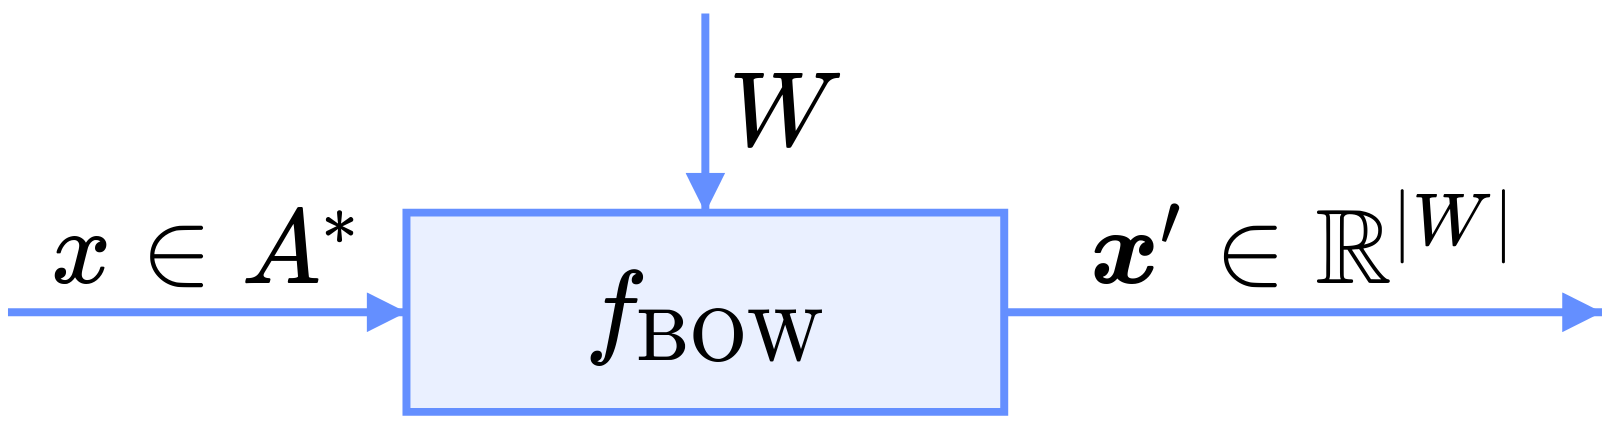
\includegraphics[width=0.9\textwidth]{assets/bow.png}
    \vspace{-0.5em}
    \captionof{figure}{BoW vectorization.}
\end{minipage}

An alternative to raw counts is using \textbf{frequencies}:
$ x'_j = \dfrac{\text{count}(w_j)}{|T|} $. 

This normalizes the vector, making the representation robust to differences in document length.

\subsubsection{TF-IDF}

A major limitation of simple BoW counting is that it highlights words that are very frequent in the corpus but not necessarily informative (e.g., the word ``good'' might appear in almost every review, making it useless for distinguishing positive from negative ones).
To address this, we use \textbf{TF-IDF} (Term Frequency-Inverse Document Frequency). It re-weights the counts to highlight words that are distinct to a specific document.
$$
\text{tfidf}(t, d, D) = \text{tf}(t, d) \cdot \text{idf}(t, D)
$$

\vspace{-1em}
Where:

\begin{minipage}{0.58\textwidth}
\begin{itemize}
    \item $t$ is the term (word);
    \item $d$ is the specific document;
    \item $D$ is the corpus (collection of all documents);
    \item $\text{tf}(t, d)$ is the \textbf{Term Frequency}: frequency of $t$ in $d$.
    \item $\text{idf}(t, D)$ is the \textbf{Inverse Document Frequency}:
    \small{
    $$
    \text{idf}(t, D) = \log \left( \frac{|D|}{|\{d \in D : t \in d\}|} \right)
    $$
    }
\end{itemize}
\end{minipage}%
\hfill
\begin{minipage}{0.40\textwidth}
    \centering
    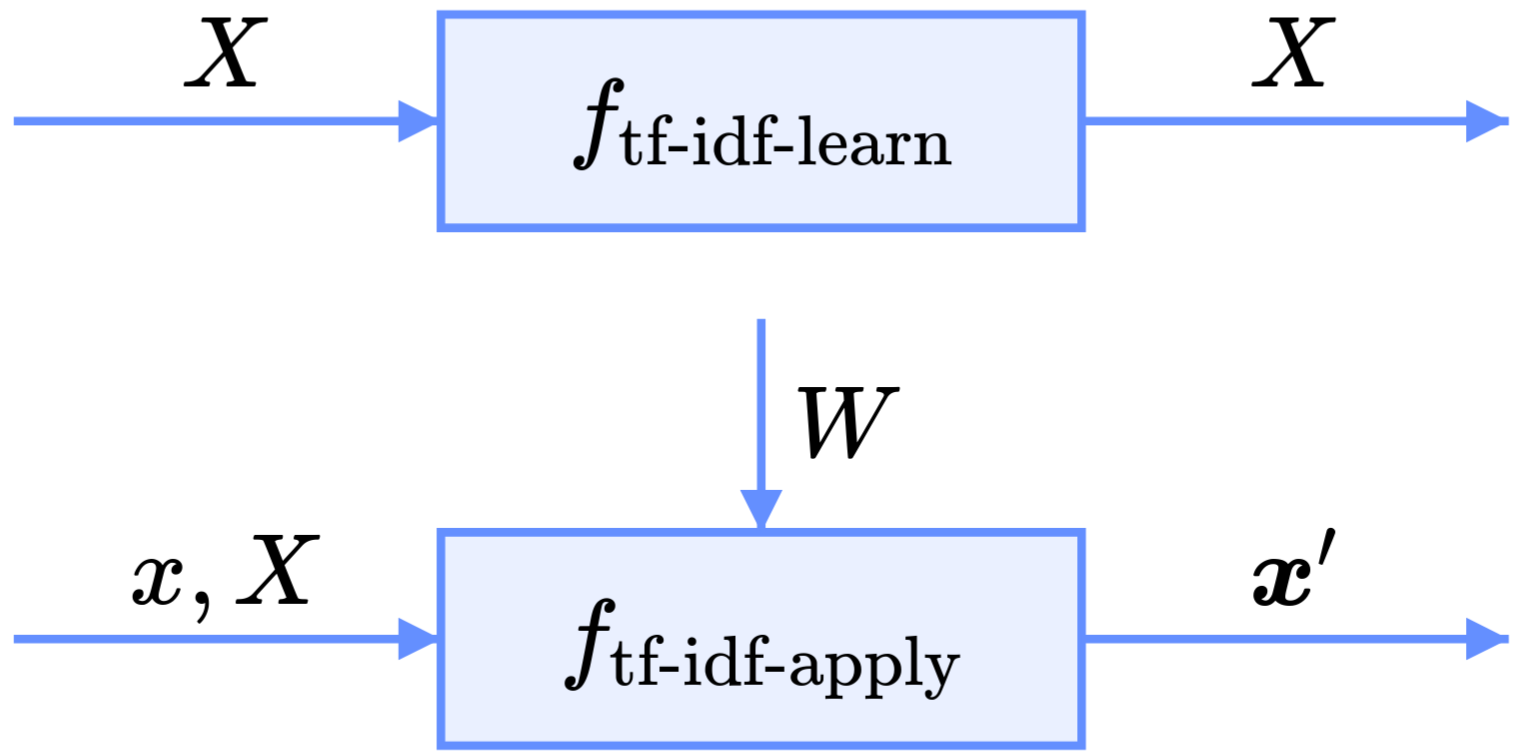
\includegraphics[width=0.9\textwidth]{assets/tf-idf.png}
    \captionof{figure}{TF-IDF logic.}
\end{minipage}

\vspace{1em}
The IDF term measures how rare the term is across the corpus. If a word appears in many documents, the ratio inside the log approaches 1, and the IDF approaches 0. Intuitively, a high TF-IDF score indicates that a word is frequent in this document but rare in the corpus, meaning it characterizes this document.

\subsubsection{Dimensionality and Context}

With BoW methods, the dimension of the input space can be huge. Common reduction practices include:
\begin{itemize}
    \item Using a very small, domain-specific dictionary.
    \item Pruning the dictionary based on frequency (e.g., keeping only the top-$k$ most frequent words).
    \item Using dimensionality reduction techniques (e.g., PCA/SVD) on the resulting matrix.
\end{itemize}

\textbf{The problem of Ordering}:
BoW destroys word order (``not bad'' becomes ``bad'' + ``not'', losing the negation context). To capture context, we can use:
\begin{itemize}
    \item \textbf{N-grams}: Instead of counting single words ($1$-grams), we count sequences of $n$ adjacent words (e.g., $2$-grams like ``not bad'', ``very good''). This captures local context but drastically increases dimensionality.
    \item \textbf{Part of Speech (POS) Tagging}: Analyzing the grammatical role (noun, verb, adjective) of words to disambiguate meaning (e.g., ``book'' as a noun vs.\ ``book'' as a verb).
\end{itemize}